\section{Jeu de données}

La création d'un jeu de données labellisé est une étape fondamentale dans le développement de modèles d'apprentissage automatique. Dans cette section, nous décrirons en détail comment nous avons constitué notre jeu de données, en nous inspirant d'une méthodologie issue d'un tutoriel de prétraitement de données séquentielles pour la classification.

\subsection{Création du Jeu de Données}
La création de notre jeu de données s'est articulée autour de deux aspects essentiels :
\begin{enumerate}
    \item Enregistrement des Données : Tout d'abord, nous avons stocké les données brutes dans des fichiers au format texte. Chacun de ces fichiers représente une session distincte de collecte de données.
    \item Attribution des Labels : Simultanément, nous avons créé un fichier de labels avec l'extension ".labels". Chaque fichier de données a été associé à un label spécifique, indiquant la nature de l'environnement ou de l'obstacle au moment de la collecte des données.
\end{enumerate}

\subsection{Consolidation des Données}
Pour rassembler l'ensemble de nos données en un seul jeu de données cohérent, nous avons fusionné tous les enregistrements dans un fichier CSV unique. Ce fichier contient toutes les données d'entrée requises pour l'entraînement et l'évaluation de nos modèles.

Le jeu de données que nous utilisons dans le cadre de cette étude a été généré à l'aide d'une application Android spécialement conçue pour collecter des données d'accéléromètre. Les données les plus récentes ont été collectées jusqu'à la date du 14 avril 2023.

\subsection{Création du Dataframe d'Accélération}
La création du dataframe à partir des données brutes d'accélération s'est déroulée en trois étapes :
\begin{enumerate}
    \item Lecture des Fichiers : Nous avons identifié tous les fichiers de données au format texte (.txt) présents dans le dossier de données.
    \item Conversion en DataFrame : Chaque fichier a été lu et converti en un DataFrame Pandas. Les données d'accélération ont été enregistrées dans les colonnes "ax", "ay", et "az". Les colonnes "file" et "index" ont été ajoutées pour enregistrer respectivement le nom du fichier source et l'indice de l'échantillon.
    \item Concaténation des DataFrames : Enfin, nous avons concaténé tous les DataFrames individuels pour obtenir un seul DataFrame global contenant l'ensemble des données d'accélération.
\end{enumerate}

Le DataFrame résultant fournit une vue d'ensemble complète des données, accompagnée de statistiques descriptives telles que la moyenne, l'écart-type, les valeurs minimales et maximales pour chaque axe d'accélération (ax, ay, az).

\subsection{Exemple de Données d'Accélération}
Voici un extrait des données d'accélération présentes dans le dataset :

\begin{figure}[h]
    \centering
    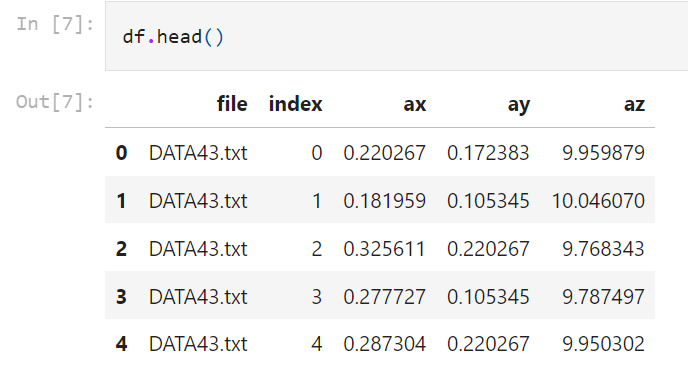
\includegraphics[width=0.4\linewidth]{img/dfhead.png}
    \caption{Extrait des données d'accélérations dans le dataset}
\end{figure}

\subsection{Création du Dataframe des Étiquettes}
Pour chaque fichier de données d'accélération, nous avons généré un label correspondant. Les labels ont été créés selon une convention simple, où chaque fichier de données est associé à un label de la forme "DATAx.txt". Par exemple, le premier fichier est associé au label "DATA1.txt", le deuxième au label "DATA2.txt", et ainsi de suite. Ces labels ont été enregistrés dans un fichier séparé nommé "DATE.labels", où chaque ligne contient le nom du fichier et son label correspondant.

\subsection{Structure du Jeu de Données}
Notre jeu de données revêt une importance capitale dans nos expérimentations. Il renferme des données d'accélération couplées à des labels, formant ainsi une base solide pour l'apprentissage automatique supervisé. Ce jeu de données joue un rôle essentiel dans l'évaluation des performances de nos modèles dans la classification des obstacles et des types de surfaces.
